\documentclass[article,12pt,onesidea,4paper,english,brazil]{abntex2}

\usepackage{lmodern, indentfirst, nomencl, color, graphicx, microtype, lipsum}			
\usepackage[T1]{fontenc}		
\usepackage[utf8]{inputenc}		

\setlrmarginsandblock{2cm}{2cm}{*}
\setulmarginsandblock{2cm}{2cm}{*}
\checkandfixthelayout

\setlength{\parindent}{1.3cm}
\setlength{\parskip}{0.2cm}

\SingleSpacing

\begin{document}
	
	\selectlanguage{brazil}
	
	\frenchspacing 
	
	\begin{center}
		\LARGE ELABORAÇÃO DE UMA MÁQUINA DE\\SOLDA ELÉTRICA COMO INSTRUMENTO DE ENSINO PARA DISCENTES
		
		\normalsize
		Diego Leônidas Esplendo Vieira\footnote{
			Orientador, diego.vieira@ifro.edu.br, IFRO – Campus Vilhena}
	Gabriel Felipe
	de Andrade Oliveira\footnote{Colaborador, gabriellegalvha@hotmail.com, IFRO – Campus Vilhena.}
	João Roberto
	Bond da Silva\footnote{Colaborador, jobond46@gmail.com, IFRO – Campus Vilhena}
	Paulo César Macedo\footnote{Co-orientador, paulo.macedo@ifro.edu.br, IFRO – CampusVilhena.}
	Ronaldo Pozzobom\footnote{
		Bolsista, ronaldopozzobom@hotmail.com, IFRO – CampusVilhena.}
	
		 
		
	\end{center}


	
	% resumo em português
	\begin{resumoumacoluna}
	Este trabalho tem o intuito de gerar um instrumento de ensino para os
	professores das disciplinas de Química, Física e Programação. Foi pesquisado
	sobre elementos que compõem uma máquina de solda e posteriormente analisado
	de acordo com o custo e benefício de cada um para a construção de uma máquina
	caseira, com o objetivo de ensinar os alunos o que foi explicado em sala de aula.
	
		\vspace{\onelineskip}
		
		\noindent
		\textbf{Palavras-chave}: Arduino. Eletrólise. Prática Didática
	\end{resumoumacoluna}
	
	\section*{Introdução}
	
	Este projeto começou com o objetivo de fabricar um instrumento de estudo
	para o ensino das disciplinas de química, física e programação. A máquina de solda
	serve como complementação do conhecimento mostrado em sala, assim o aluno
	poderá ver na prática o que foi explicado pelo professor, já que a Instituição possuía
	poucos materiais de ensino fabricados pelos alunos. No processo de confecção da
	máquina foram utilizados alguns componentes químicos e realizados alguns estudos
	específicos para conseguirmos um resultado plausível, que será discutido
	posteriormente neste artigo. Um segundo objetivo é trazer a correlação dos cursos
	de técnico em Informática e Eletromecânica do IFRO Campus Vilhena, pois o projeto
	possui alunos dos dois cursos.
	
	\section*{Material e Método}
	
	Para que houvesse uma economia na hora da fabricação da máquina, os
	alunos ficaram responsáveis por pesquisar quais os melhores materiais para utilizar
	na máquina, levando em conta o custo e o benefício que cada um deles traria. Os
	principais materiais utilizados foram cobre, sal de cozinha (Cloreto de Sódio/NaCl),
	água natural e placas de acrílico de 5 milímetros de espessura. Para que a máquina
	ficasse automatizada, foi utilizado Arduino, componentes de leitura do Arduino, eixo
	liso para que os eletrodos possam correr dentro da solução e rolamentos axiais.
	A metodologia foi muito simples, porém totalmente produtiva. Os alunos
	ficaram responsáveis por fazer pesquisas sobre os materiais como aqui já dito e
	também sobre eletrônica básica, pois todo conhecimento sobre a área era
	necessário. Após esta etapa, os participantes do projeto começaram a montagem da
	caixa de acrílico, onde a substância que conduz a energia fica. Logo em seguida, foi
	a montagem dos mecanismos de automação da máquina.
	
	\section*{Resultados e Discussão}
	Ao iniciar a pesquisa, foram feitos alguns testes para que pudéssemos definir
	qual seria a melhor solução para utilizar na eletrólise, já que a mesma não iria gerar
	energia, apenas a conduziria, “injetando” uma certa quantia de elétrons pelo seu
	polo negativo e “aspirando” a mesma quantia pelo polo positivo.(FELTRE,2005)
	Após as pesquisas e testes, encontramos alguns valores (Tabela 1) que
	constataram que o cloreto de sódio (NaCl) seria a melhor substância para se utilizar
	na máquina mesmo não sendo o melhor condutor, por conta de a relação custobenefício ser maior que o hidróxido de sódio que é complicado de ser encontrado e
	possui um preço bem maior que o cloreto de sódio.
	
	\begin{figure}[h]
		\centering
		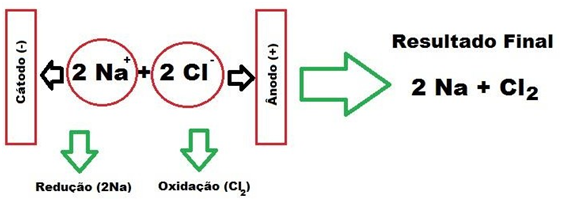
\includegraphics[width=0.7\linewidth]{pip-67-1}
		\caption{ Processo de eletrólise do cloreto de sódio. IFRO, 2015.}
		\label{fig:pip-67-1}
	\end{figure}
Na figura 1, temos uma simulação de como a eletrólise vai ocorrer dentro de
uma cuba com água (HO). Os eletrodos representados na imagem (ânodo (+) e
cátodo (-)) são de cobre e a solução é a mistura da água da cuba com o cloreto de
sódio (NaCl). Após a dissociação dos íons, ocorre os processos de redução e
oxidação.

Na fase da redução, o cloro (cátion) está precisando de dois elétrons para ficar
neutro e recebe os elétrons do cátodo, gerando o 2Na.

Já na fase de oxidação, o sódio (ânion) possui dois elétrons em excesso e
precisa ficar neutro. Para que isso ocorra, os elétrons que estão sobrando vão para
o ânodo, onde este os envia para o polo negativo por haver uma diferença de
potencial. O resultado é o Cl$_2$.

Ao encerrar os processos de oxidação e redução, obtemos cloro e sódio
metálico (2Na + Cl$_2$).

Os eletrodos utilizados foram placas de cobre, onde novamente encontramos o
melhor custo-benefício, pois a platina e o ouro que são os melhores condutores no
mercado atualmente possuem um preço muito alto, assim, a possibilidade de utilizar
esses metais foi descartada.

A caixa foi feita toda de acrílico onde a mesma vai servir de cuba eletrolítica e
possui dois eixos que guiam um dos eletrodos, como na figura 2. Os dois eixos
horizontais servem de sustentação e guia para mover a plataforma com os eletrodos
acoplados. Conectado a plataforma móvel há uma malha de cobre que serve de
cabo terra, que permite a condução de energia(fase).

Na parte fixa, há conectado ao eletrodo o cabo. As plataformas possuem
movimentos longitudinais proporcionados por quatro rolamentos axiais, os
rolamentos são componentes mecânicos com baixo coeficiente de atrito estático e
cinético. Por outro lado, a parte fixa utiliza os rolamentos somente como
estabilizador.

\begin{figure}[h]
	\centering
	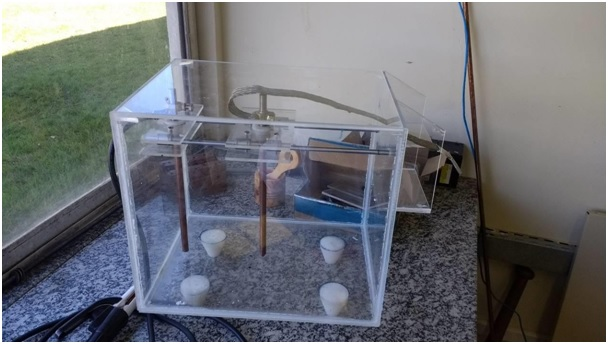
\includegraphics[width=0.7\linewidth]{pip-68-01}
	\caption{Máquina de solda elétrica em construção. IFRO, 2015}
	\label{fig:pip-68-01}
\end{figure}

Após toda a fase de construção da caixa, foram feitos testes para ver se a
solda que a máquina estava fazendo era relativamente boa antes de colocar os
componentes do Arduino. Para o teste usamos uma tensão de 46,7 V e foi preciso de uma solução de concentração 4 Kg (quilogramas) de NaCl (Cloreto
de Sódio) + 20 L (litros) de HO (Água). O teste foi um sucesso, derretendo
eletrodos 6013 de 2,5 mm (milímetros), com corrente inicial de 46A (Ampére) e
final de 64A onde a mesma varia linearmente. Vimos também que não houve
nenhum vazamento da solução e que toda a vedação que foi feita com silicone
estava de acordo.

A parte da automação veio em seguida, onde colocamos todos os
componentes do Arduino em seus devidos lugares. Foi utilizado um Arduino
Uno R3, motor de passo nema 17 e um display simples com botões. Já na
programação, foram feitas estruturas condicionais utilizando o resultado que
vem do sensor de amperagem, assim, o usuário consegue definir uma
amperagem para a soldagem.

A automação da máquina teve uma ajuda grande dos alunos de
informática que fazem parte do projeto, mostrando que dentro da instituição há
uma integração entre os cursos para um bem maior.

O uso de micro controladores Atmel (Arduino) para o ensino da física
também já foi citado em alguns projetos, principalmente onde Souza (2011)
enfatiza que os kits montados por grandes empresas são caros, dificultando a
aquisição do material e que com o Arduino seria capaz de trazer o mesmo
conhecimento, porém com um investimento menor.

Portanto, temos um kit relativamente barato para mostrar na prática como
funciona o processo de eletrólise.

	\section*{Conclusões}
	
	Percebemos que as aplicações para este projeto seriam principalmente para
	fins didáticos, mas também poderia ser usado para pequenos reparos na Instituição.
	Com a máquina o aluno poderá aprender, na prática, conceitos que foram vistos na
	sala de aula, fazendo com que o mesmo desenvolva cada vez mais a capacidade de
	pesquisar sobre a área. Futuramente, seria interessante fazer outras máquinas
	como a que foi construída, assim, a Instituição teria mais materiais para ensinar os
	alunos

	\section*{Instituição de Fomento}
	A instituição de fomento foi o IFRO – Campus Vilhena, que possibilitou a
	realização deste projeto.
	
	\section*{Referências}
	
	\noindent FELTRE, Ricardo Arissa. Fundamentos da Química. 4. ed. São Paulo: Moderna,
	2005. 700 p. 428
	SOUZA, Anderson R. de. A placa Arduino: uma opção de baixo custo para
	experiências de física assistidas pelo PC. Revista Brasileira de Ensino de
	Física, SãoPaulo,v.33,n.1,p.01-05,jan.2011.Disponívelem:
	<http://dx.doi.org/10.1590/S1806-11172011000100026.>. Acesso em: 05 jul. 2016.
\end{document}
